\documentclass[14pt,letterpaper]{extarticle}
\usepackage[T1]{fontenc}
\usepackage[utf8]{inputenc}
\usepackage{helvet}
\renewcommand{\familydefault}{\sfdefault}
\usepackage[letterpaper,landscape,left=0.75in,right=0.75in,top=0.85in,bottom=0.85in,headheight=18pt,headsep=14pt,footskip=26pt]{geometry}
\usepackage{tikz}
\usepackage{pifont}
\usepackage{fancyhdr}
\definecolor{cred}{RGB}{214,39,40}
\definecolor{cblue}{RGB}{31,92,204}
\pagestyle{fancy}
\fancyhf{}
\renewcommand{\headrulewidth}{0pt}
\lhead{Week NN / Patterns you cannot avoid / Grades K--1}
\lfoot{Bellingham Math Circle / Week NN / NN-K-v1}
\rfoot{\thepage}
\setlength{\parindent}{0pt}
\setlength{\parskip}{4pt}
\linespread{1.12}
\begin{document}
Put a red or a blue counter on every square of a strip. The strip is good if a comb never shows three counters of one color, wherever you slide it.
\vspace{-4pt}\begin{center}
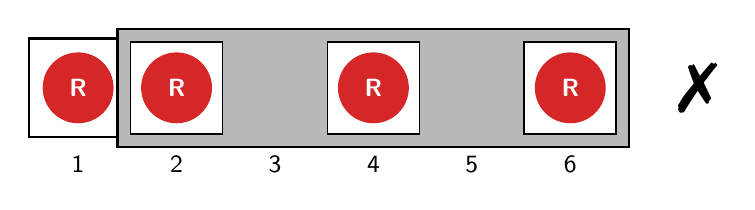
\begin{tikzpicture}
\draw[line width=0.9pt] (0.000,0.000) rectangle (1.250,1.250);
\node[font=\small, anchor=base] at (0.625,-0.450) {1};
\draw[line width=0.9pt] (1.250,0.000) rectangle (2.500,1.250);
\node[font=\small, anchor=base] at (1.875,-0.450) {2};
\draw[line width=0.9pt] (2.500,0.000) rectangle (3.750,1.250);
\node[font=\small, anchor=base] at (3.125,-0.450) {3};
\draw[line width=0.9pt] (3.750,0.000) rectangle (5.000,1.250);
\node[font=\small, anchor=base] at (4.375,-0.450) {4};
\draw[line width=0.9pt] (5.000,0.000) rectangle (6.250,1.250);
\node[font=\small, anchor=base] at (5.625,-0.450) {5};
\draw[line width=0.9pt] (6.250,0.000) rectangle (7.500,1.250);
\node[font=\small, anchor=base] at (6.875,-0.450) {6};
\fill[cred] (0.625,0.625) circle (0.450);\node[text=white,font=\bfseries\small] at (0.625,0.625) {R};
\fill[cred] (1.875,0.625) circle (0.450);\node[text=white,font=\bfseries\small] at (1.875,0.625) {R};
\fill[cblue] (3.125,0.625) circle (0.450);\node[text=white,font=\bfseries\small] at (3.125,0.625) {B};
\fill[cred] (4.375,0.625) circle (0.450);\node[text=white,font=\bfseries\small] at (4.375,0.625) {R};
\fill[cblue] (5.625,0.625) circle (0.450);\node[text=white,font=\bfseries\small] at (5.625,0.625) {B};
\fill[cred] (6.875,0.625) circle (0.450);\node[text=white,font=\bfseries\small] at (6.875,0.625) {R};
\fill[gray!55, even odd rule] (1.125,-0.125) rectangle (7.625,1.375) (1.290,0.040) rectangle (2.460,1.210) (3.790,0.040) rectangle (4.960,1.210) (6.290,0.040) rectangle (7.460,1.210);
\draw[line width=0.8pt] (1.125,-0.125) rectangle (7.625,1.375);
\draw[line width=0.6pt] (1.290,0.040) rectangle (2.460,1.210);
\draw[line width=0.6pt] (3.790,0.040) rectangle (4.960,1.210);
\draw[line width=0.6pt] (6.290,0.040) rectangle (7.460,1.210);
\node[font=\Huge] at (8.500,0.625) {\ding{55}};
\end{tikzpicture}
\end{center}
\vspace{2pt}
\par\noindent\textbf{Problem 1:} Make each strip good, then color it.\par

\vspace{2pt}\begin{center}
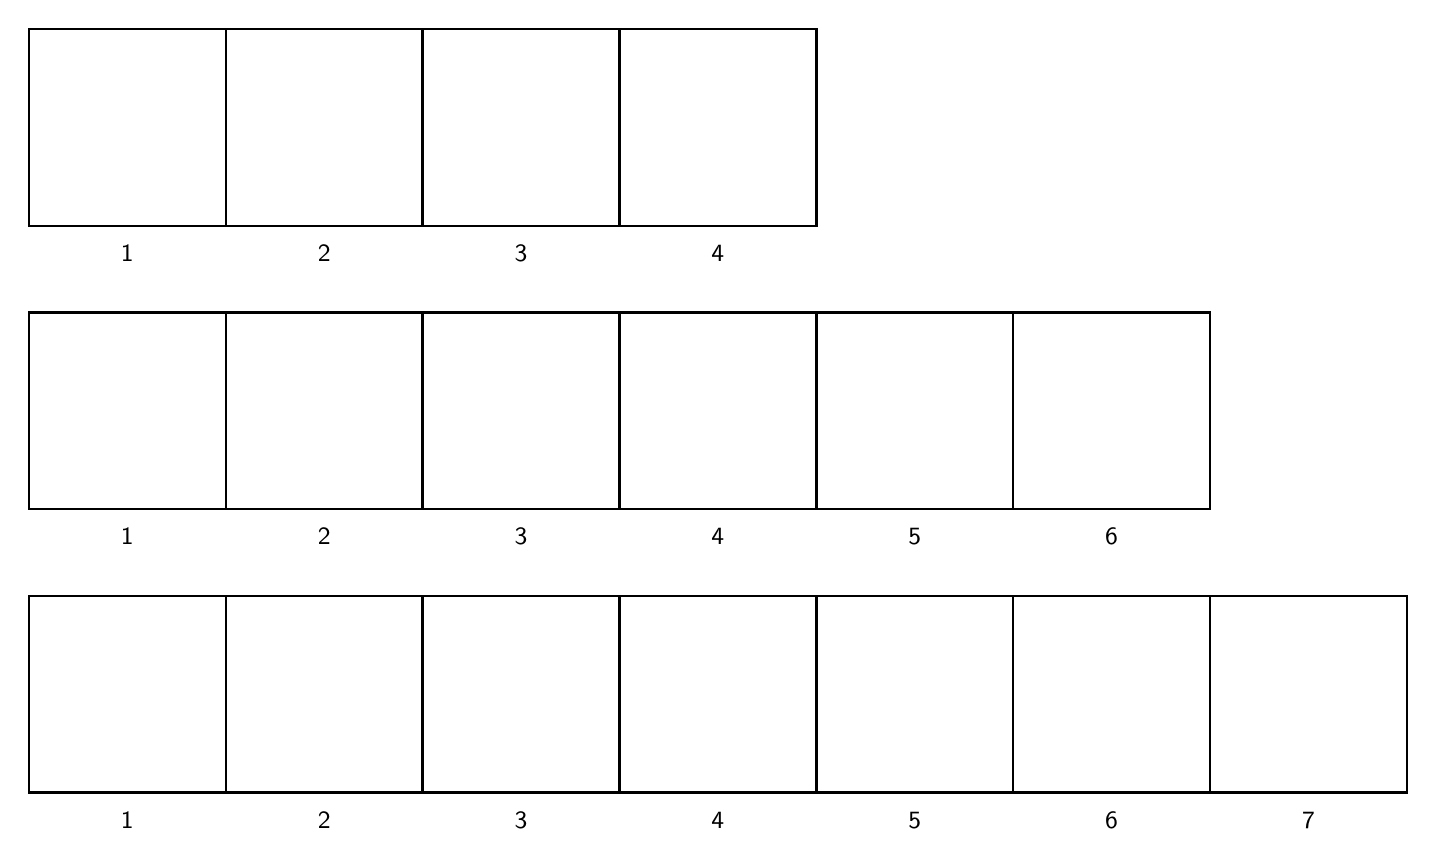
\begin{tikzpicture}
\draw[line width=0.9pt] (0.000,0.000) rectangle (2.500,2.500);
\node[font=\small, anchor=base] at (1.250,-0.450) {1};
\draw[line width=0.9pt] (2.500,0.000) rectangle (5.000,2.500);
\node[font=\small, anchor=base] at (3.750,-0.450) {2};
\draw[line width=0.9pt] (5.000,0.000) rectangle (7.500,2.500);
\node[font=\small, anchor=base] at (6.250,-0.450) {3};
\draw[line width=0.9pt] (7.500,0.000) rectangle (10.000,2.500);
\node[font=\small, anchor=base] at (8.750,-0.450) {4};
\draw[line width=0.9pt] (0.000,-3.600) rectangle (2.500,-1.100);
\node[font=\small, anchor=base] at (1.250,-4.050) {1};
\draw[line width=0.9pt] (2.500,-3.600) rectangle (5.000,-1.100);
\node[font=\small, anchor=base] at (3.750,-4.050) {2};
\draw[line width=0.9pt] (5.000,-3.600) rectangle (7.500,-1.100);
\node[font=\small, anchor=base] at (6.250,-4.050) {3};
\draw[line width=0.9pt] (7.500,-3.600) rectangle (10.000,-1.100);
\node[font=\small, anchor=base] at (8.750,-4.050) {4};
\draw[line width=0.9pt] (10.000,-3.600) rectangle (12.500,-1.100);
\node[font=\small, anchor=base] at (11.250,-4.050) {5};
\draw[line width=0.9pt] (12.500,-3.600) rectangle (15.000,-1.100);
\node[font=\small, anchor=base] at (13.750,-4.050) {6};
\draw[line width=0.9pt] (0.000,-7.200) rectangle (2.500,-4.700);
\node[font=\small, anchor=base] at (1.250,-7.650) {1};
\draw[line width=0.9pt] (2.500,-7.200) rectangle (5.000,-4.700);
\node[font=\small, anchor=base] at (3.750,-7.650) {2};
\draw[line width=0.9pt] (5.000,-7.200) rectangle (7.500,-4.700);
\node[font=\small, anchor=base] at (6.250,-7.650) {3};
\draw[line width=0.9pt] (7.500,-7.200) rectangle (10.000,-4.700);
\node[font=\small, anchor=base] at (8.750,-7.650) {4};
\draw[line width=0.9pt] (10.000,-7.200) rectangle (12.500,-4.700);
\node[font=\small, anchor=base] at (11.250,-7.650) {5};
\draw[line width=0.9pt] (12.500,-7.200) rectangle (15.000,-4.700);
\node[font=\small, anchor=base] at (13.750,-7.650) {6};
\draw[line width=0.9pt] (15.000,-7.200) rectangle (17.500,-4.700);
\node[font=\small, anchor=base] at (16.250,-7.650) {7};
\end{tikzpicture}
\end{center}
\newpage
\par\noindent\textbf{Problem 2:} Finish each strip so that it is good.\par

\vspace{2pt}\begin{center}
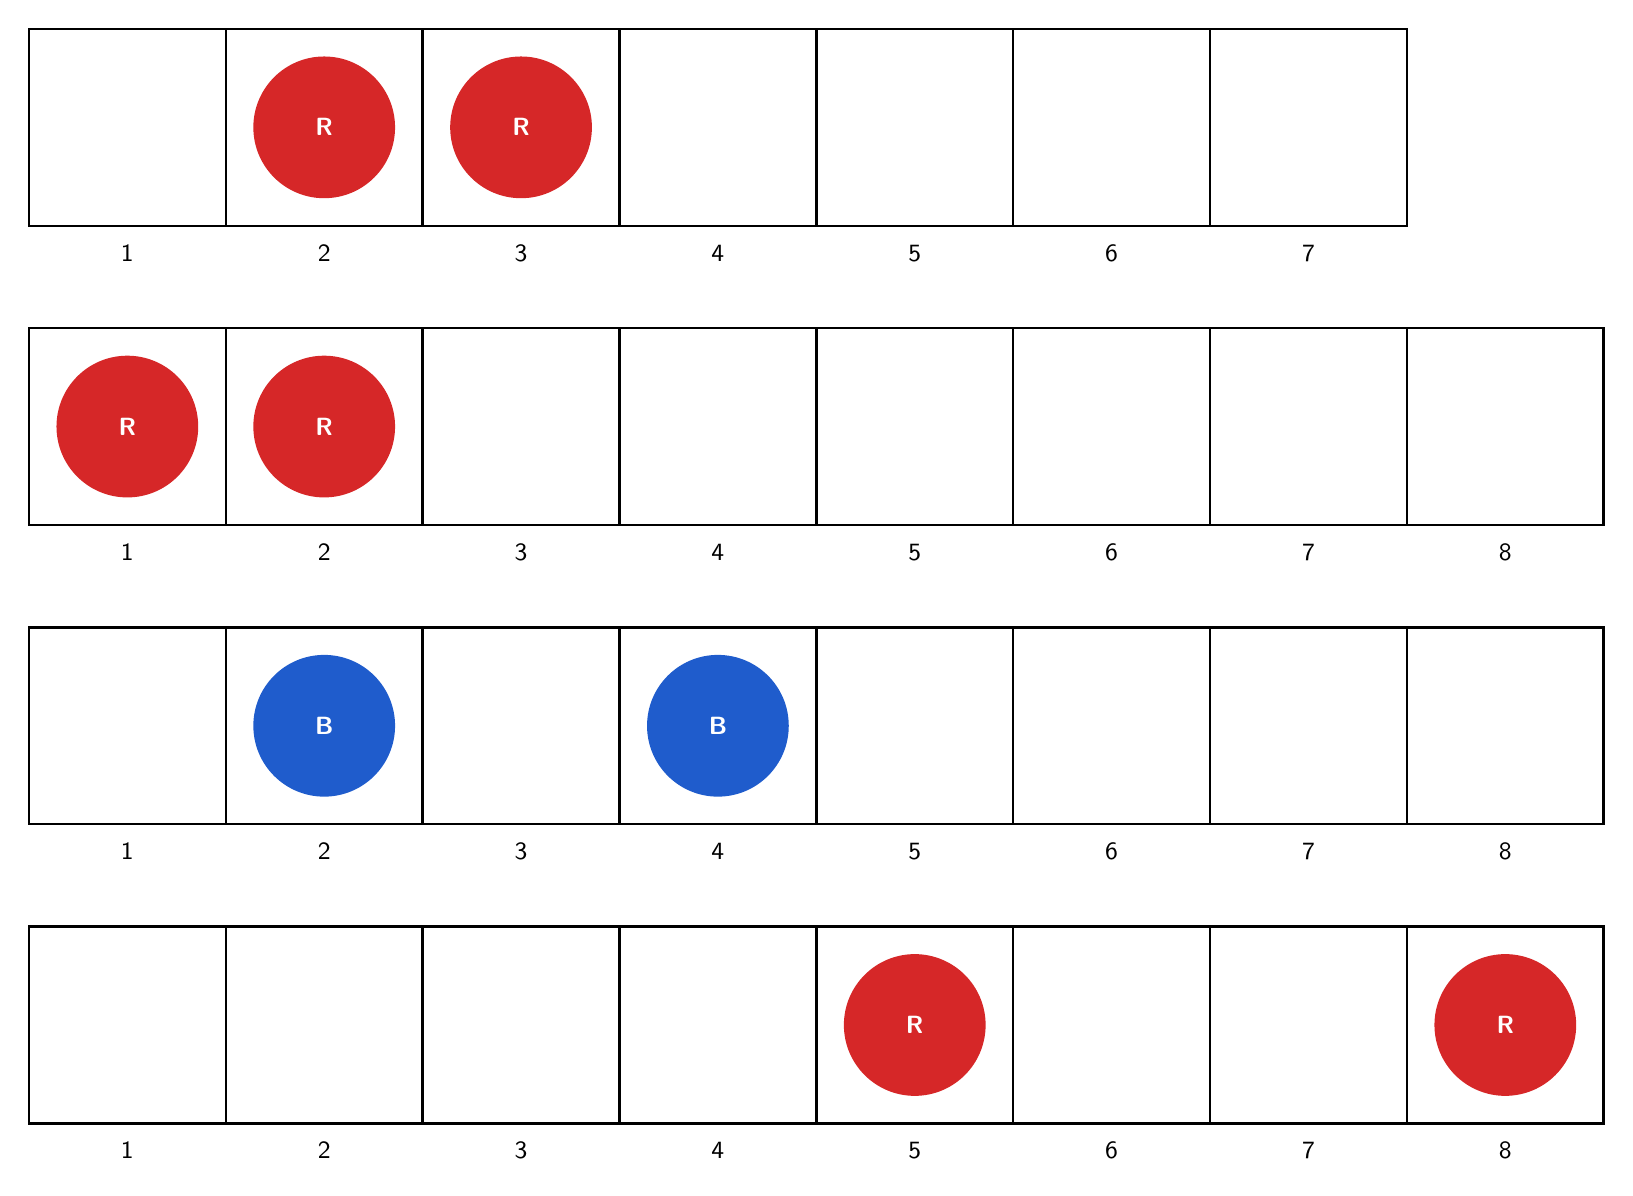
\begin{tikzpicture}
\draw[line width=0.9pt] (0.000,0.000) rectangle (2.500,2.500);
\node[font=\small, anchor=base] at (1.250,-0.450) {1};
\draw[line width=0.9pt] (2.500,0.000) rectangle (5.000,2.500);
\node[font=\small, anchor=base] at (3.750,-0.450) {2};
\draw[line width=0.9pt] (5.000,0.000) rectangle (7.500,2.500);
\node[font=\small, anchor=base] at (6.250,-0.450) {3};
\draw[line width=0.9pt] (7.500,0.000) rectangle (10.000,2.500);
\node[font=\small, anchor=base] at (8.750,-0.450) {4};
\draw[line width=0.9pt] (10.000,0.000) rectangle (12.500,2.500);
\node[font=\small, anchor=base] at (11.250,-0.450) {5};
\draw[line width=0.9pt] (12.500,0.000) rectangle (15.000,2.500);
\node[font=\small, anchor=base] at (13.750,-0.450) {6};
\draw[line width=0.9pt] (15.000,0.000) rectangle (17.500,2.500);
\node[font=\small, anchor=base] at (16.250,-0.450) {7};
\fill[cred] (3.750,1.250) circle (0.900);\node[text=white,font=\bfseries\small] at (3.750,1.250) {R};
\fill[cred] (6.250,1.250) circle (0.900);\node[text=white,font=\bfseries\small] at (6.250,1.250) {R};
\draw[line width=0.9pt] (0.000,-3.800) rectangle (2.500,-1.300);
\node[font=\small, anchor=base] at (1.250,-4.250) {1};
\draw[line width=0.9pt] (2.500,-3.800) rectangle (5.000,-1.300);
\node[font=\small, anchor=base] at (3.750,-4.250) {2};
\draw[line width=0.9pt] (5.000,-3.800) rectangle (7.500,-1.300);
\node[font=\small, anchor=base] at (6.250,-4.250) {3};
\draw[line width=0.9pt] (7.500,-3.800) rectangle (10.000,-1.300);
\node[font=\small, anchor=base] at (8.750,-4.250) {4};
\draw[line width=0.9pt] (10.000,-3.800) rectangle (12.500,-1.300);
\node[font=\small, anchor=base] at (11.250,-4.250) {5};
\draw[line width=0.9pt] (12.500,-3.800) rectangle (15.000,-1.300);
\node[font=\small, anchor=base] at (13.750,-4.250) {6};
\draw[line width=0.9pt] (15.000,-3.800) rectangle (17.500,-1.300);
\node[font=\small, anchor=base] at (16.250,-4.250) {7};
\draw[line width=0.9pt] (17.500,-3.800) rectangle (20.000,-1.300);
\node[font=\small, anchor=base] at (18.750,-4.250) {8};
\fill[cred] (1.250,-2.550) circle (0.900);\node[text=white,font=\bfseries\small] at (1.250,-2.550) {R};
\fill[cred] (3.750,-2.550) circle (0.900);\node[text=white,font=\bfseries\small] at (3.750,-2.550) {R};
\draw[line width=0.9pt] (0.000,-7.600) rectangle (2.500,-5.100);
\node[font=\small, anchor=base] at (1.250,-8.050) {1};
\draw[line width=0.9pt] (2.500,-7.600) rectangle (5.000,-5.100);
\node[font=\small, anchor=base] at (3.750,-8.050) {2};
\draw[line width=0.9pt] (5.000,-7.600) rectangle (7.500,-5.100);
\node[font=\small, anchor=base] at (6.250,-8.050) {3};
\draw[line width=0.9pt] (7.500,-7.600) rectangle (10.000,-5.100);
\node[font=\small, anchor=base] at (8.750,-8.050) {4};
\draw[line width=0.9pt] (10.000,-7.600) rectangle (12.500,-5.100);
\node[font=\small, anchor=base] at (11.250,-8.050) {5};
\draw[line width=0.9pt] (12.500,-7.600) rectangle (15.000,-5.100);
\node[font=\small, anchor=base] at (13.750,-8.050) {6};
\draw[line width=0.9pt] (15.000,-7.600) rectangle (17.500,-5.100);
\node[font=\small, anchor=base] at (16.250,-8.050) {7};
\draw[line width=0.9pt] (17.500,-7.600) rectangle (20.000,-5.100);
\node[font=\small, anchor=base] at (18.750,-8.050) {8};
\fill[cblue] (3.750,-6.350) circle (0.900);\node[text=white,font=\bfseries\small] at (3.750,-6.350) {B};
\fill[cblue] (8.750,-6.350) circle (0.900);\node[text=white,font=\bfseries\small] at (8.750,-6.350) {B};
\draw[line width=0.9pt] (0.000,-11.400) rectangle (2.500,-8.900);
\node[font=\small, anchor=base] at (1.250,-11.850) {1};
\draw[line width=0.9pt] (2.500,-11.400) rectangle (5.000,-8.900);
\node[font=\small, anchor=base] at (3.750,-11.850) {2};
\draw[line width=0.9pt] (5.000,-11.400) rectangle (7.500,-8.900);
\node[font=\small, anchor=base] at (6.250,-11.850) {3};
\draw[line width=0.9pt] (7.500,-11.400) rectangle (10.000,-8.900);
\node[font=\small, anchor=base] at (8.750,-11.850) {4};
\draw[line width=0.9pt] (10.000,-11.400) rectangle (12.500,-8.900);
\node[font=\small, anchor=base] at (11.250,-11.850) {5};
\draw[line width=0.9pt] (12.500,-11.400) rectangle (15.000,-8.900);
\node[font=\small, anchor=base] at (13.750,-11.850) {6};
\draw[line width=0.9pt] (15.000,-11.400) rectangle (17.500,-8.900);
\node[font=\small, anchor=base] at (16.250,-11.850) {7};
\draw[line width=0.9pt] (17.500,-11.400) rectangle (20.000,-8.900);
\node[font=\small, anchor=base] at (18.750,-11.850) {8};
\fill[cred] (11.250,-10.150) circle (0.900);\node[text=white,font=\bfseries\small] at (11.250,-10.150) {R};
\fill[cred] (18.750,-10.150) circle (0.900);\node[text=white,font=\bfseries\small] at (18.750,-10.150) {R};
\end{tikzpicture}
\end{center}
\newpage
\par\noindent\textbf{Problem 3:} Make the strip of 8 squares good. Can you make the strip of 9 squares good?\par

\vspace{6pt}\begin{center}
\begin{tikzpicture}
\draw[line width=0.9pt] (0.000,0.000) rectangle (2.500,2.500);
\node[font=\small, anchor=base] at (1.250,-0.450) {1};
\draw[line width=0.9pt] (2.500,0.000) rectangle (5.000,2.500);
\node[font=\small, anchor=base] at (3.750,-0.450) {2};
\draw[line width=0.9pt] (5.000,0.000) rectangle (7.500,2.500);
\node[font=\small, anchor=base] at (6.250,-0.450) {3};
\draw[line width=0.9pt] (7.500,0.000) rectangle (10.000,2.500);
\node[font=\small, anchor=base] at (8.750,-0.450) {4};
\draw[line width=0.9pt] (10.000,0.000) rectangle (12.500,2.500);
\node[font=\small, anchor=base] at (11.250,-0.450) {5};
\draw[line width=0.9pt] (12.500,0.000) rectangle (15.000,2.500);
\node[font=\small, anchor=base] at (13.750,-0.450) {6};
\draw[line width=0.9pt] (15.000,0.000) rectangle (17.500,2.500);
\node[font=\small, anchor=base] at (16.250,-0.450) {7};
\draw[line width=0.9pt] (17.500,0.000) rectangle (20.000,2.500);
\node[font=\small, anchor=base] at (18.750,-0.450) {8};
\draw[line width=0.9pt] (0.000,-4.700) rectangle (2.500,-2.200);
\node[font=\small, anchor=base] at (1.250,-5.150) {1};
\draw[line width=0.9pt] (2.500,-4.700) rectangle (5.000,-2.200);
\node[font=\small, anchor=base] at (3.750,-5.150) {2};
\draw[line width=0.9pt] (5.000,-4.700) rectangle (7.500,-2.200);
\node[font=\small, anchor=base] at (6.250,-5.150) {3};
\draw[line width=0.9pt] (7.500,-4.700) rectangle (10.000,-2.200);
\node[font=\small, anchor=base] at (8.750,-5.150) {4};
\draw[line width=0.9pt] (10.000,-4.700) rectangle (12.500,-2.200);
\node[font=\small, anchor=base] at (11.250,-5.150) {5};
\draw[line width=0.9pt] (12.500,-4.700) rectangle (15.000,-2.200);
\node[font=\small, anchor=base] at (13.750,-5.150) {6};
\draw[line width=0.9pt] (15.000,-4.700) rectangle (17.500,-2.200);
\node[font=\small, anchor=base] at (16.250,-5.150) {7};
\draw[line width=0.9pt] (17.500,-4.700) rectangle (20.000,-2.200);
\node[font=\small, anchor=base] at (18.750,-5.150) {8};
\draw[line width=0.9pt] (20.000,-4.700) rectangle (22.500,-2.200);
\node[font=\small, anchor=base] at (21.250,-5.150) {9};
\end{tikzpicture}
\end{center}
\newpage
\par\noindent\textbf{Problem 4:} Play against the adult or a partner on the strip of 9 squares. Take turns putting a red or a blue counter on an empty square. Check with the combs after every turn. If a comb shows three counters of one color, the player who just moved loses.\par

\vspace{2pt}\begin{center}
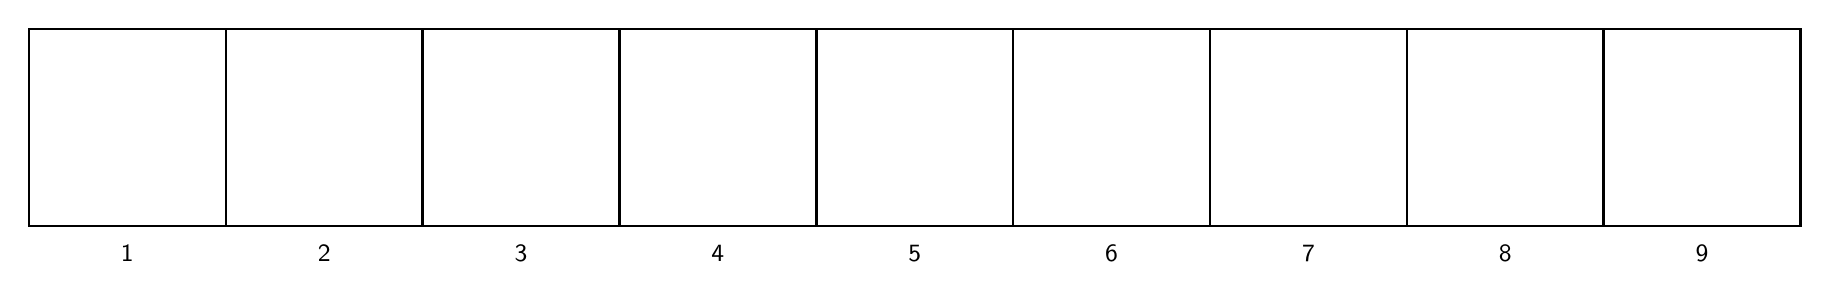
\begin{tikzpicture}
\draw[line width=0.9pt] (0.000,0.000) rectangle (2.500,2.500);
\node[font=\small, anchor=base] at (1.250,-0.450) {1};
\draw[line width=0.9pt] (2.500,0.000) rectangle (5.000,2.500);
\node[font=\small, anchor=base] at (3.750,-0.450) {2};
\draw[line width=0.9pt] (5.000,0.000) rectangle (7.500,2.500);
\node[font=\small, anchor=base] at (6.250,-0.450) {3};
\draw[line width=0.9pt] (7.500,0.000) rectangle (10.000,2.500);
\node[font=\small, anchor=base] at (8.750,-0.450) {4};
\draw[line width=0.9pt] (10.000,0.000) rectangle (12.500,2.500);
\node[font=\small, anchor=base] at (11.250,-0.450) {5};
\draw[line width=0.9pt] (12.500,0.000) rectangle (15.000,2.500);
\node[font=\small, anchor=base] at (13.750,-0.450) {6};
\draw[line width=0.9pt] (15.000,0.000) rectangle (17.500,2.500);
\node[font=\small, anchor=base] at (16.250,-0.450) {7};
\draw[line width=0.9pt] (17.500,0.000) rectangle (20.000,2.500);
\node[font=\small, anchor=base] at (18.750,-0.450) {8};
\draw[line width=0.9pt] (20.000,0.000) rectangle (22.500,2.500);
\node[font=\small, anchor=base] at (21.250,-0.450) {9};
\end{tikzpicture}
\end{center}
\vspace{1.4cm}
\par\noindent\textbf{Problem 5:} Play the same game on the strip of 8 squares. Can a game end with all the squares filled and nobody losing? On the strip of 9 squares, would you rather go first or second?\par

\vspace{2pt}\begin{center}
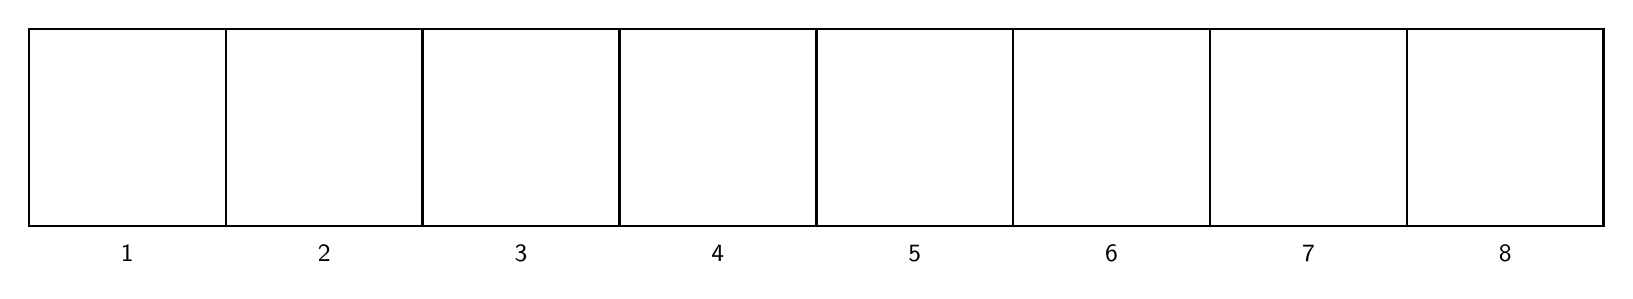
\begin{tikzpicture}
\draw[line width=0.9pt] (0.000,0.000) rectangle (2.500,2.500);
\node[font=\small, anchor=base] at (1.250,-0.450) {1};
\draw[line width=0.9pt] (2.500,0.000) rectangle (5.000,2.500);
\node[font=\small, anchor=base] at (3.750,-0.450) {2};
\draw[line width=0.9pt] (5.000,0.000) rectangle (7.500,2.500);
\node[font=\small, anchor=base] at (6.250,-0.450) {3};
\draw[line width=0.9pt] (7.500,0.000) rectangle (10.000,2.500);
\node[font=\small, anchor=base] at (8.750,-0.450) {4};
\draw[line width=0.9pt] (10.000,0.000) rectangle (12.500,2.500);
\node[font=\small, anchor=base] at (11.250,-0.450) {5};
\draw[line width=0.9pt] (12.500,0.000) rectangle (15.000,2.500);
\node[font=\small, anchor=base] at (13.750,-0.450) {6};
\draw[line width=0.9pt] (15.000,0.000) rectangle (17.500,2.500);
\node[font=\small, anchor=base] at (16.250,-0.450) {7};
\draw[line width=0.9pt] (17.500,0.000) rectangle (20.000,2.500);
\node[font=\small, anchor=base] at (18.750,-0.450) {8};
\end{tikzpicture}
\end{center}
\newpage
\par\noindent\textbf{Problem 6:} Find every good strip of 8 squares.\par

\vspace{2pt}\begin{center}
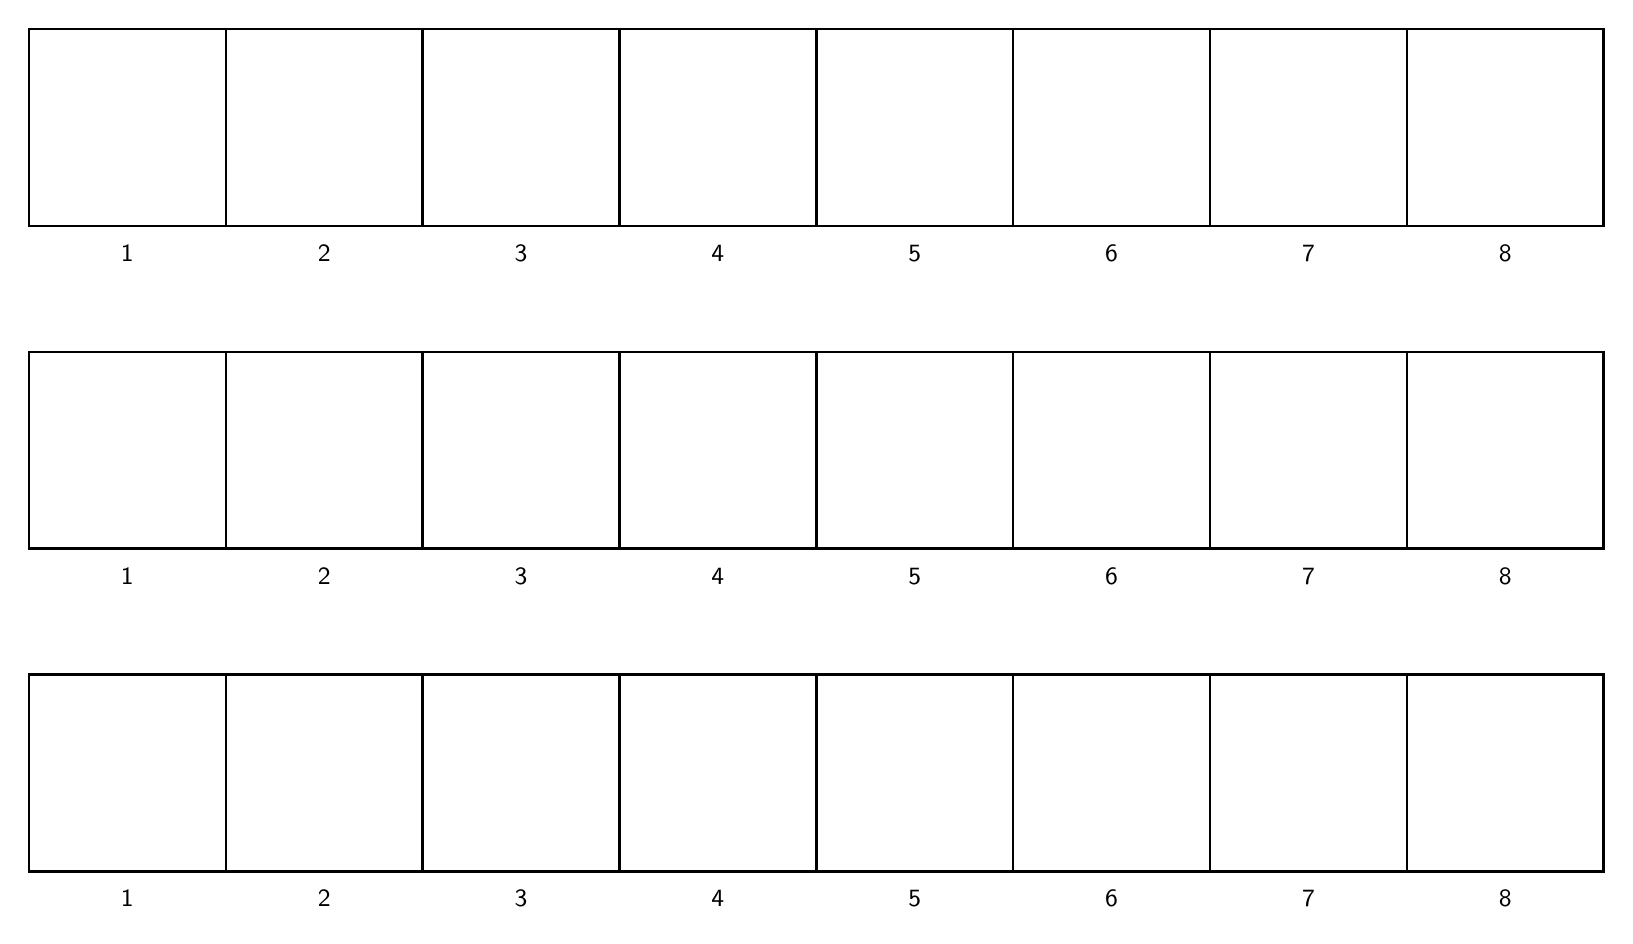
\begin{tikzpicture}
\draw[line width=0.9pt] (0.000,0.000) rectangle (2.500,2.500);
\node[font=\small, anchor=base] at (1.250,-0.450) {1};
\draw[line width=0.9pt] (2.500,0.000) rectangle (5.000,2.500);
\node[font=\small, anchor=base] at (3.750,-0.450) {2};
\draw[line width=0.9pt] (5.000,0.000) rectangle (7.500,2.500);
\node[font=\small, anchor=base] at (6.250,-0.450) {3};
\draw[line width=0.9pt] (7.500,0.000) rectangle (10.000,2.500);
\node[font=\small, anchor=base] at (8.750,-0.450) {4};
\draw[line width=0.9pt] (10.000,0.000) rectangle (12.500,2.500);
\node[font=\small, anchor=base] at (11.250,-0.450) {5};
\draw[line width=0.9pt] (12.500,0.000) rectangle (15.000,2.500);
\node[font=\small, anchor=base] at (13.750,-0.450) {6};
\draw[line width=0.9pt] (15.000,0.000) rectangle (17.500,2.500);
\node[font=\small, anchor=base] at (16.250,-0.450) {7};
\draw[line width=0.9pt] (17.500,0.000) rectangle (20.000,2.500);
\node[font=\small, anchor=base] at (18.750,-0.450) {8};
\draw[line width=0.9pt] (0.000,-4.100) rectangle (2.500,-1.600);
\node[font=\small, anchor=base] at (1.250,-4.550) {1};
\draw[line width=0.9pt] (2.500,-4.100) rectangle (5.000,-1.600);
\node[font=\small, anchor=base] at (3.750,-4.550) {2};
\draw[line width=0.9pt] (5.000,-4.100) rectangle (7.500,-1.600);
\node[font=\small, anchor=base] at (6.250,-4.550) {3};
\draw[line width=0.9pt] (7.500,-4.100) rectangle (10.000,-1.600);
\node[font=\small, anchor=base] at (8.750,-4.550) {4};
\draw[line width=0.9pt] (10.000,-4.100) rectangle (12.500,-1.600);
\node[font=\small, anchor=base] at (11.250,-4.550) {5};
\draw[line width=0.9pt] (12.500,-4.100) rectangle (15.000,-1.600);
\node[font=\small, anchor=base] at (13.750,-4.550) {6};
\draw[line width=0.9pt] (15.000,-4.100) rectangle (17.500,-1.600);
\node[font=\small, anchor=base] at (16.250,-4.550) {7};
\draw[line width=0.9pt] (17.500,-4.100) rectangle (20.000,-1.600);
\node[font=\small, anchor=base] at (18.750,-4.550) {8};
\draw[line width=0.9pt] (0.000,-8.200) rectangle (2.500,-5.700);
\node[font=\small, anchor=base] at (1.250,-8.650) {1};
\draw[line width=0.9pt] (2.500,-8.200) rectangle (5.000,-5.700);
\node[font=\small, anchor=base] at (3.750,-8.650) {2};
\draw[line width=0.9pt] (5.000,-8.200) rectangle (7.500,-5.700);
\node[font=\small, anchor=base] at (6.250,-8.650) {3};
\draw[line width=0.9pt] (7.500,-8.200) rectangle (10.000,-5.700);
\node[font=\small, anchor=base] at (8.750,-8.650) {4};
\draw[line width=0.9pt] (10.000,-8.200) rectangle (12.500,-5.700);
\node[font=\small, anchor=base] at (11.250,-8.650) {5};
\draw[line width=0.9pt] (12.500,-8.200) rectangle (15.000,-5.700);
\node[font=\small, anchor=base] at (13.750,-8.650) {6};
\draw[line width=0.9pt] (15.000,-8.200) rectangle (17.500,-5.700);
\node[font=\small, anchor=base] at (16.250,-8.650) {7};
\draw[line width=0.9pt] (17.500,-8.200) rectangle (20.000,-5.700);
\node[font=\small, anchor=base] at (18.750,-8.650) {8};
\end{tikzpicture}
\end{center}
\newpage
More strips for Problem 6.\par\vspace{2pt}\begin{center}
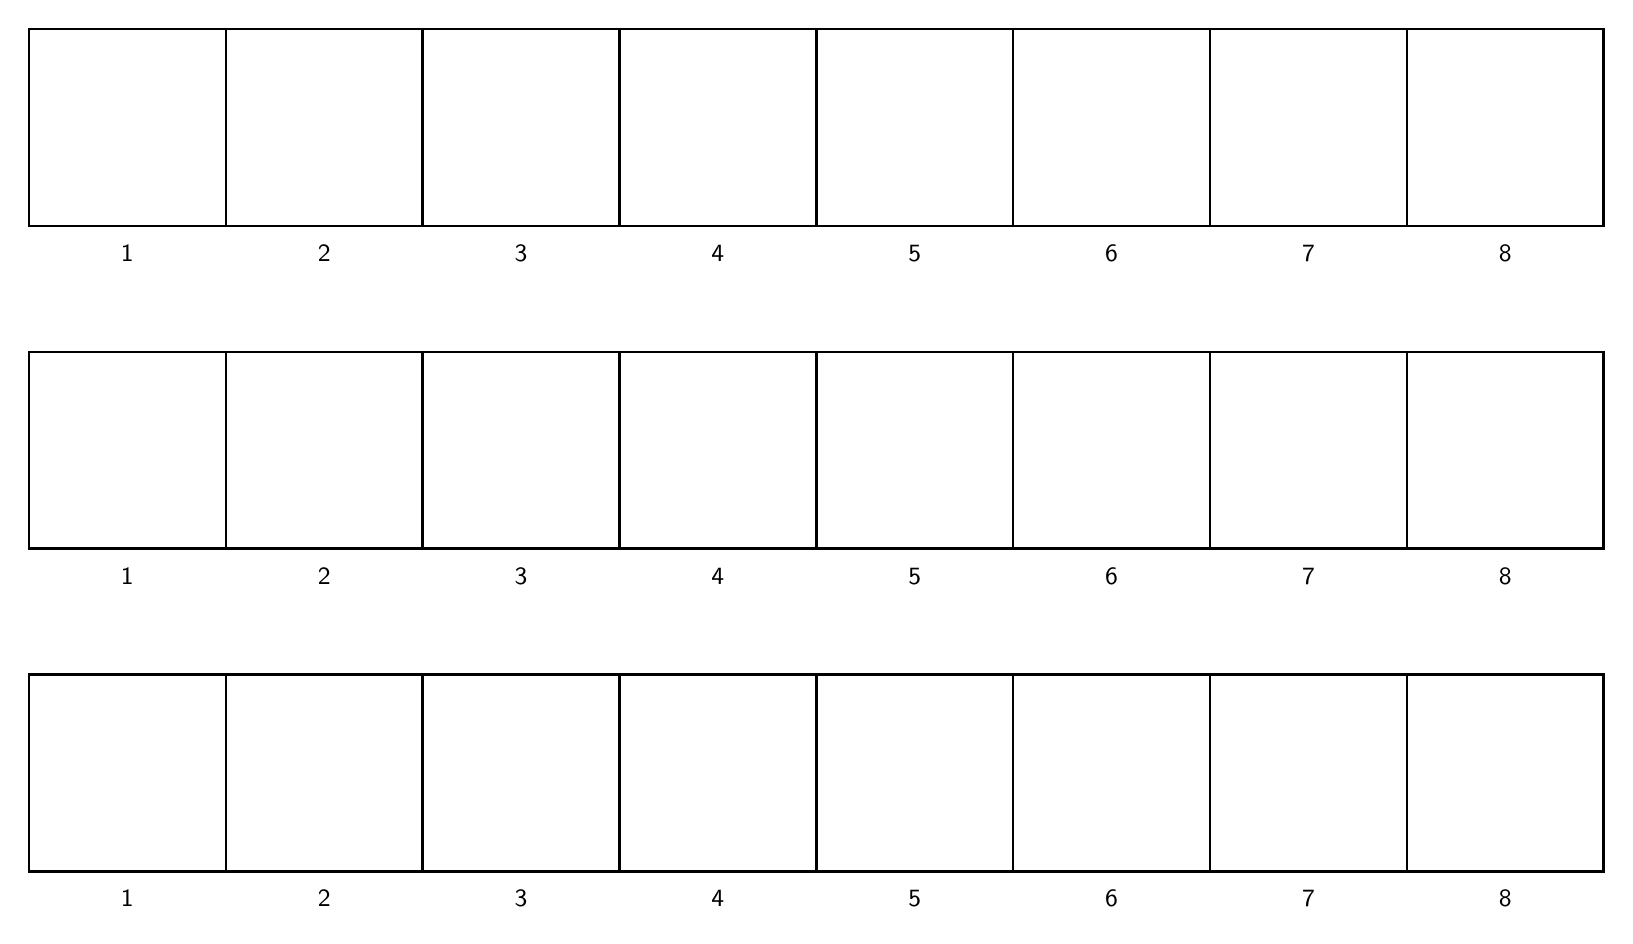
\begin{tikzpicture}
\draw[line width=0.9pt] (0.000,0.000) rectangle (2.500,2.500);
\node[font=\small, anchor=base] at (1.250,-0.450) {1};
\draw[line width=0.9pt] (2.500,0.000) rectangle (5.000,2.500);
\node[font=\small, anchor=base] at (3.750,-0.450) {2};
\draw[line width=0.9pt] (5.000,0.000) rectangle (7.500,2.500);
\node[font=\small, anchor=base] at (6.250,-0.450) {3};
\draw[line width=0.9pt] (7.500,0.000) rectangle (10.000,2.500);
\node[font=\small, anchor=base] at (8.750,-0.450) {4};
\draw[line width=0.9pt] (10.000,0.000) rectangle (12.500,2.500);
\node[font=\small, anchor=base] at (11.250,-0.450) {5};
\draw[line width=0.9pt] (12.500,0.000) rectangle (15.000,2.500);
\node[font=\small, anchor=base] at (13.750,-0.450) {6};
\draw[line width=0.9pt] (15.000,0.000) rectangle (17.500,2.500);
\node[font=\small, anchor=base] at (16.250,-0.450) {7};
\draw[line width=0.9pt] (17.500,0.000) rectangle (20.000,2.500);
\node[font=\small, anchor=base] at (18.750,-0.450) {8};
\draw[line width=0.9pt] (0.000,-4.100) rectangle (2.500,-1.600);
\node[font=\small, anchor=base] at (1.250,-4.550) {1};
\draw[line width=0.9pt] (2.500,-4.100) rectangle (5.000,-1.600);
\node[font=\small, anchor=base] at (3.750,-4.550) {2};
\draw[line width=0.9pt] (5.000,-4.100) rectangle (7.500,-1.600);
\node[font=\small, anchor=base] at (6.250,-4.550) {3};
\draw[line width=0.9pt] (7.500,-4.100) rectangle (10.000,-1.600);
\node[font=\small, anchor=base] at (8.750,-4.550) {4};
\draw[line width=0.9pt] (10.000,-4.100) rectangle (12.500,-1.600);
\node[font=\small, anchor=base] at (11.250,-4.550) {5};
\draw[line width=0.9pt] (12.500,-4.100) rectangle (15.000,-1.600);
\node[font=\small, anchor=base] at (13.750,-4.550) {6};
\draw[line width=0.9pt] (15.000,-4.100) rectangle (17.500,-1.600);
\node[font=\small, anchor=base] at (16.250,-4.550) {7};
\draw[line width=0.9pt] (17.500,-4.100) rectangle (20.000,-1.600);
\node[font=\small, anchor=base] at (18.750,-4.550) {8};
\draw[line width=0.9pt] (0.000,-8.200) rectangle (2.500,-5.700);
\node[font=\small, anchor=base] at (1.250,-8.650) {1};
\draw[line width=0.9pt] (2.500,-8.200) rectangle (5.000,-5.700);
\node[font=\small, anchor=base] at (3.750,-8.650) {2};
\draw[line width=0.9pt] (5.000,-8.200) rectangle (7.500,-5.700);
\node[font=\small, anchor=base] at (6.250,-8.650) {3};
\draw[line width=0.9pt] (7.500,-8.200) rectangle (10.000,-5.700);
\node[font=\small, anchor=base] at (8.750,-8.650) {4};
\draw[line width=0.9pt] (10.000,-8.200) rectangle (12.500,-5.700);
\node[font=\small, anchor=base] at (11.250,-8.650) {5};
\draw[line width=0.9pt] (12.500,-8.200) rectangle (15.000,-5.700);
\node[font=\small, anchor=base] at (13.750,-8.650) {6};
\draw[line width=0.9pt] (15.000,-8.200) rectangle (17.500,-5.700);
\node[font=\small, anchor=base] at (16.250,-8.650) {7};
\draw[line width=0.9pt] (17.500,-8.200) rectangle (20.000,-5.700);
\node[font=\small, anchor=base] at (18.750,-8.650) {8};
\end{tikzpicture}
\end{center}
\end{document}
